\section{Topological data analysis}
\label{sec:topological-data-analysis}
\textit{Topological Data Analysis} (TDA) is a fast-growing field of mathematics, providing a set of tools from topology to infer underlying features from data \cite{chazal2021introduction}. In this section, we will introduce relevant concepts from TDA. In particular, we will introduce the simplicial complex in \cref{sec:simplicial-complex} and persistence diagrams in \cref{sec:persistence diagram}. Furthermore, we will introduce a method for vectorizing persistence diagrams, namely the persistence image in \cref{sec:persistence-image}, and a commonly used distance metric for persistence diagrams, namely the $p$-Wasserstein distance in \cref{sec:wasserstein-distance}. Finally, we will introduce two algorithms that uses concepts from TDA to identify singular words (or data points), namely topological polysemy in \cref{sec:topological-polysemy} and Geometric Anomaly Detection in \cref{sec:geometric-anomaly-detection}. This section is based on \cites{Edelsbrunner2010}{chazal2021introduction}, if not stated otherwise.

\subsection{Simplicial complex}
\label{sec:simplicial-complex}
In computer science, a \textit{graph} is a datatype for describing possibly non-linear and complex relationships between data points. In particular, graphs consist of vertices and edges, where the edges connect the vertices. Edges can also have metadata such as weight and direction. A common graph to use (in the context of computer science) is the $k$-nearest neighbour graph, where vertices are data points and edges represent neighbouring relationships, with distance as weight. A \textit{simplicial complex} is a generalization of graphs and we see its particular usage in TDA, due to its topological properties. Simplicial complexes consist of \textit{$n$-simplices}, where $0$-simplices are similar to vertices, $1$-simplices are similar to edges. The difference between graphs and simplicial complexes occur when we look at $n$-simplices for $n \geq 2$. For example, $2$-simplices form triangles and $3$-simplices form tetrahedrons (i.e. triangular pyramids). We show examples of $n$-simplices in \cref{fig:n-simplices-example}.
\begin{figure}[H]
    \centering
    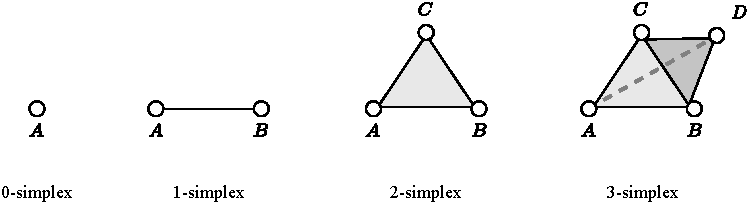
\includegraphics[width=0.9\textwidth]{thesis/figures/n-simplices_cropped.pdf}
    \caption{Building blocks of simplicial complexes, consisting of $n$-simplices.}
    \label{fig:n-simplices-example}
\end{figure}
By combining one or more $n$-simplices, we form simplicial complexes. We illustrate an example of a simplicial complex in \cref{fig:simplicial-complex}.
\begin{figure}[H]
    \centering
    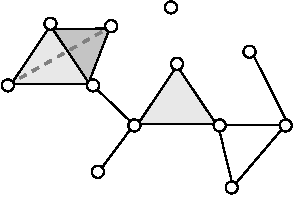
\includegraphics[width=0.5\textwidth]{thesis/figures/simplicial-complex_cropped.pdf}
    \caption{Simplicial complex consisting of $0$-, $1$-, $2$- and $3$-simplices.}
    \label{fig:simplicial-complex}
\end{figure}
There exist several methods for creating simplicial complexes from data. In particular, we look at one such simplicial complex in the next sub-subsection, namely the Vietoris–Rips complex.

\subsubsection{Vietoris–Rips complex}
\label{sec:vietoris-rips-complex}
The \textit{Vietoris–Rips complex} is a simplicial complex that we create from data points using any distance metric. Let $\alpha$ be a \textit{proximity diameter}. We build the Vietoris–Rips complex by forming a simplex for every set of $k$ data points with distance less than or equal to $\alpha$. That is, if $k$ data points satisfy $d(x_i, x_j) \leq \alpha$ (where $d(x_i, x_j)$ computes the distance between two data points $i$ and $j$), we create a $(k-1)$ simplex for that particular data point (1-simplex for two data points, 2-simplex for three data points, etc.). We illustrate with an example of a Vietoris–Rips complex in \cref{fig:simplicial-complex-rips}.
\begin{figure}[H]
    \centering
    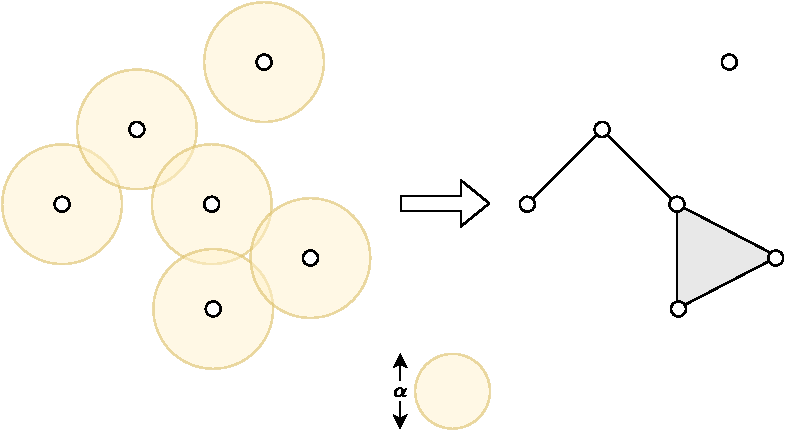
\includegraphics[width=0.7\textwidth]{thesis/figures/simplicial-complex-rips_cropped.pdf}
    \caption{A Vietoris–Rips complex on 2-dimensional data with proximity diameter $\alpha$.}
    \label{fig:simplicial-complex-rips}
\end{figure}
By carefully studying the $n$-simplices of a Vietoris–Rips complex, we can observe topological structures such as \textit{loops} (i.e. $2$-simplices) or \textit{holes}  (i.e. $3$-simplices). We show an example of a loop in \cref{fig:simplicial-complex-rips}, where the rightmost data points that the bottom form a 2-simplex. To study the topological properties of data, it is common to look at varying values of $\alpha$, starting at zero and increasing to infinity. In particular, we use what we call \textit{persistent homology}, which is the study of observing how the topology changes once a threshold (e.g. $\alpha$) increases. To easily present and visualize persistent homology, we use persistence diagrams. We look at persistence diagrams in the next subsection.

\subsection{Persistence diagram}
\label{sec:persistence diagram}
To present persistent homology of a simplicial complex, we use \textit{persistence diagrams}. In persistence diagrams, we look at a range of proximity diameters over multiple persistent \textit{homology dimensions} (or \textit{homology degrees}), where the dimension refer to which $n$-simplices we want to look at (0-dimensional persistent homology observe changes of $0$-simplices, 1-dimensional observe changes of $1$-simplices, etc.). A persistence diagram is 2-dimensional, where the x-axis denotes the birth time and the y-axis the death time. Assuming that we want to create a persistence diagram of data points, we let the proximity diameter $\alpha$ start at zero. By gradually increasing $\alpha$, new topological properties appear and old topological properties merge into other properties. In particular, once a topological property is "birthed" (e.g. 1-simplex between two data points), the birth time is noted for the particular data point. A point in the persistence diagram appears once $n$-simplices merge into new $m$-simplices (e.g. three 1-simplex becoming a 2-simplex).

To motivate the use of persistence diagrams, we illustrate with a simple example in \cref{fig:persistence-diagram-example}, where we study the change of 0-dimensional persistent homology. In \cref{fig:persistence-diagram-example}, we see how the persistence diagram changes once we increase the proximity diameter $\alpha$, on a data set consisting of two blobs. In \cref{fig:persistence-diagram-example} (a), we let $\alpha=0.2$ and we observe that there are only two data points intersecting, thus leading to a single point in the persistence diagram. In \cref{fig:persistence-diagram-example} (b), we let $\alpha=1.5$ and we observe how the data points in each blob connect, thus leading to several entries in the persistence diagram. In \cref{fig:persistence-diagram-example} (c), we let $\alpha=4.5$, and we observe that there is a single point and several points on the bottom in the persistence diagram. By looking at the plot on the left, we see how the two blobs intersect and all data points have connections to other data points with distance less or equal to $\alpha$. In addition to this, \cref{fig:persistence-diagram-example} (c) indicates that we have two clusters in our data, although our data is rather noisy and could be more compact.
\begin{figure}[H]
    \centering
    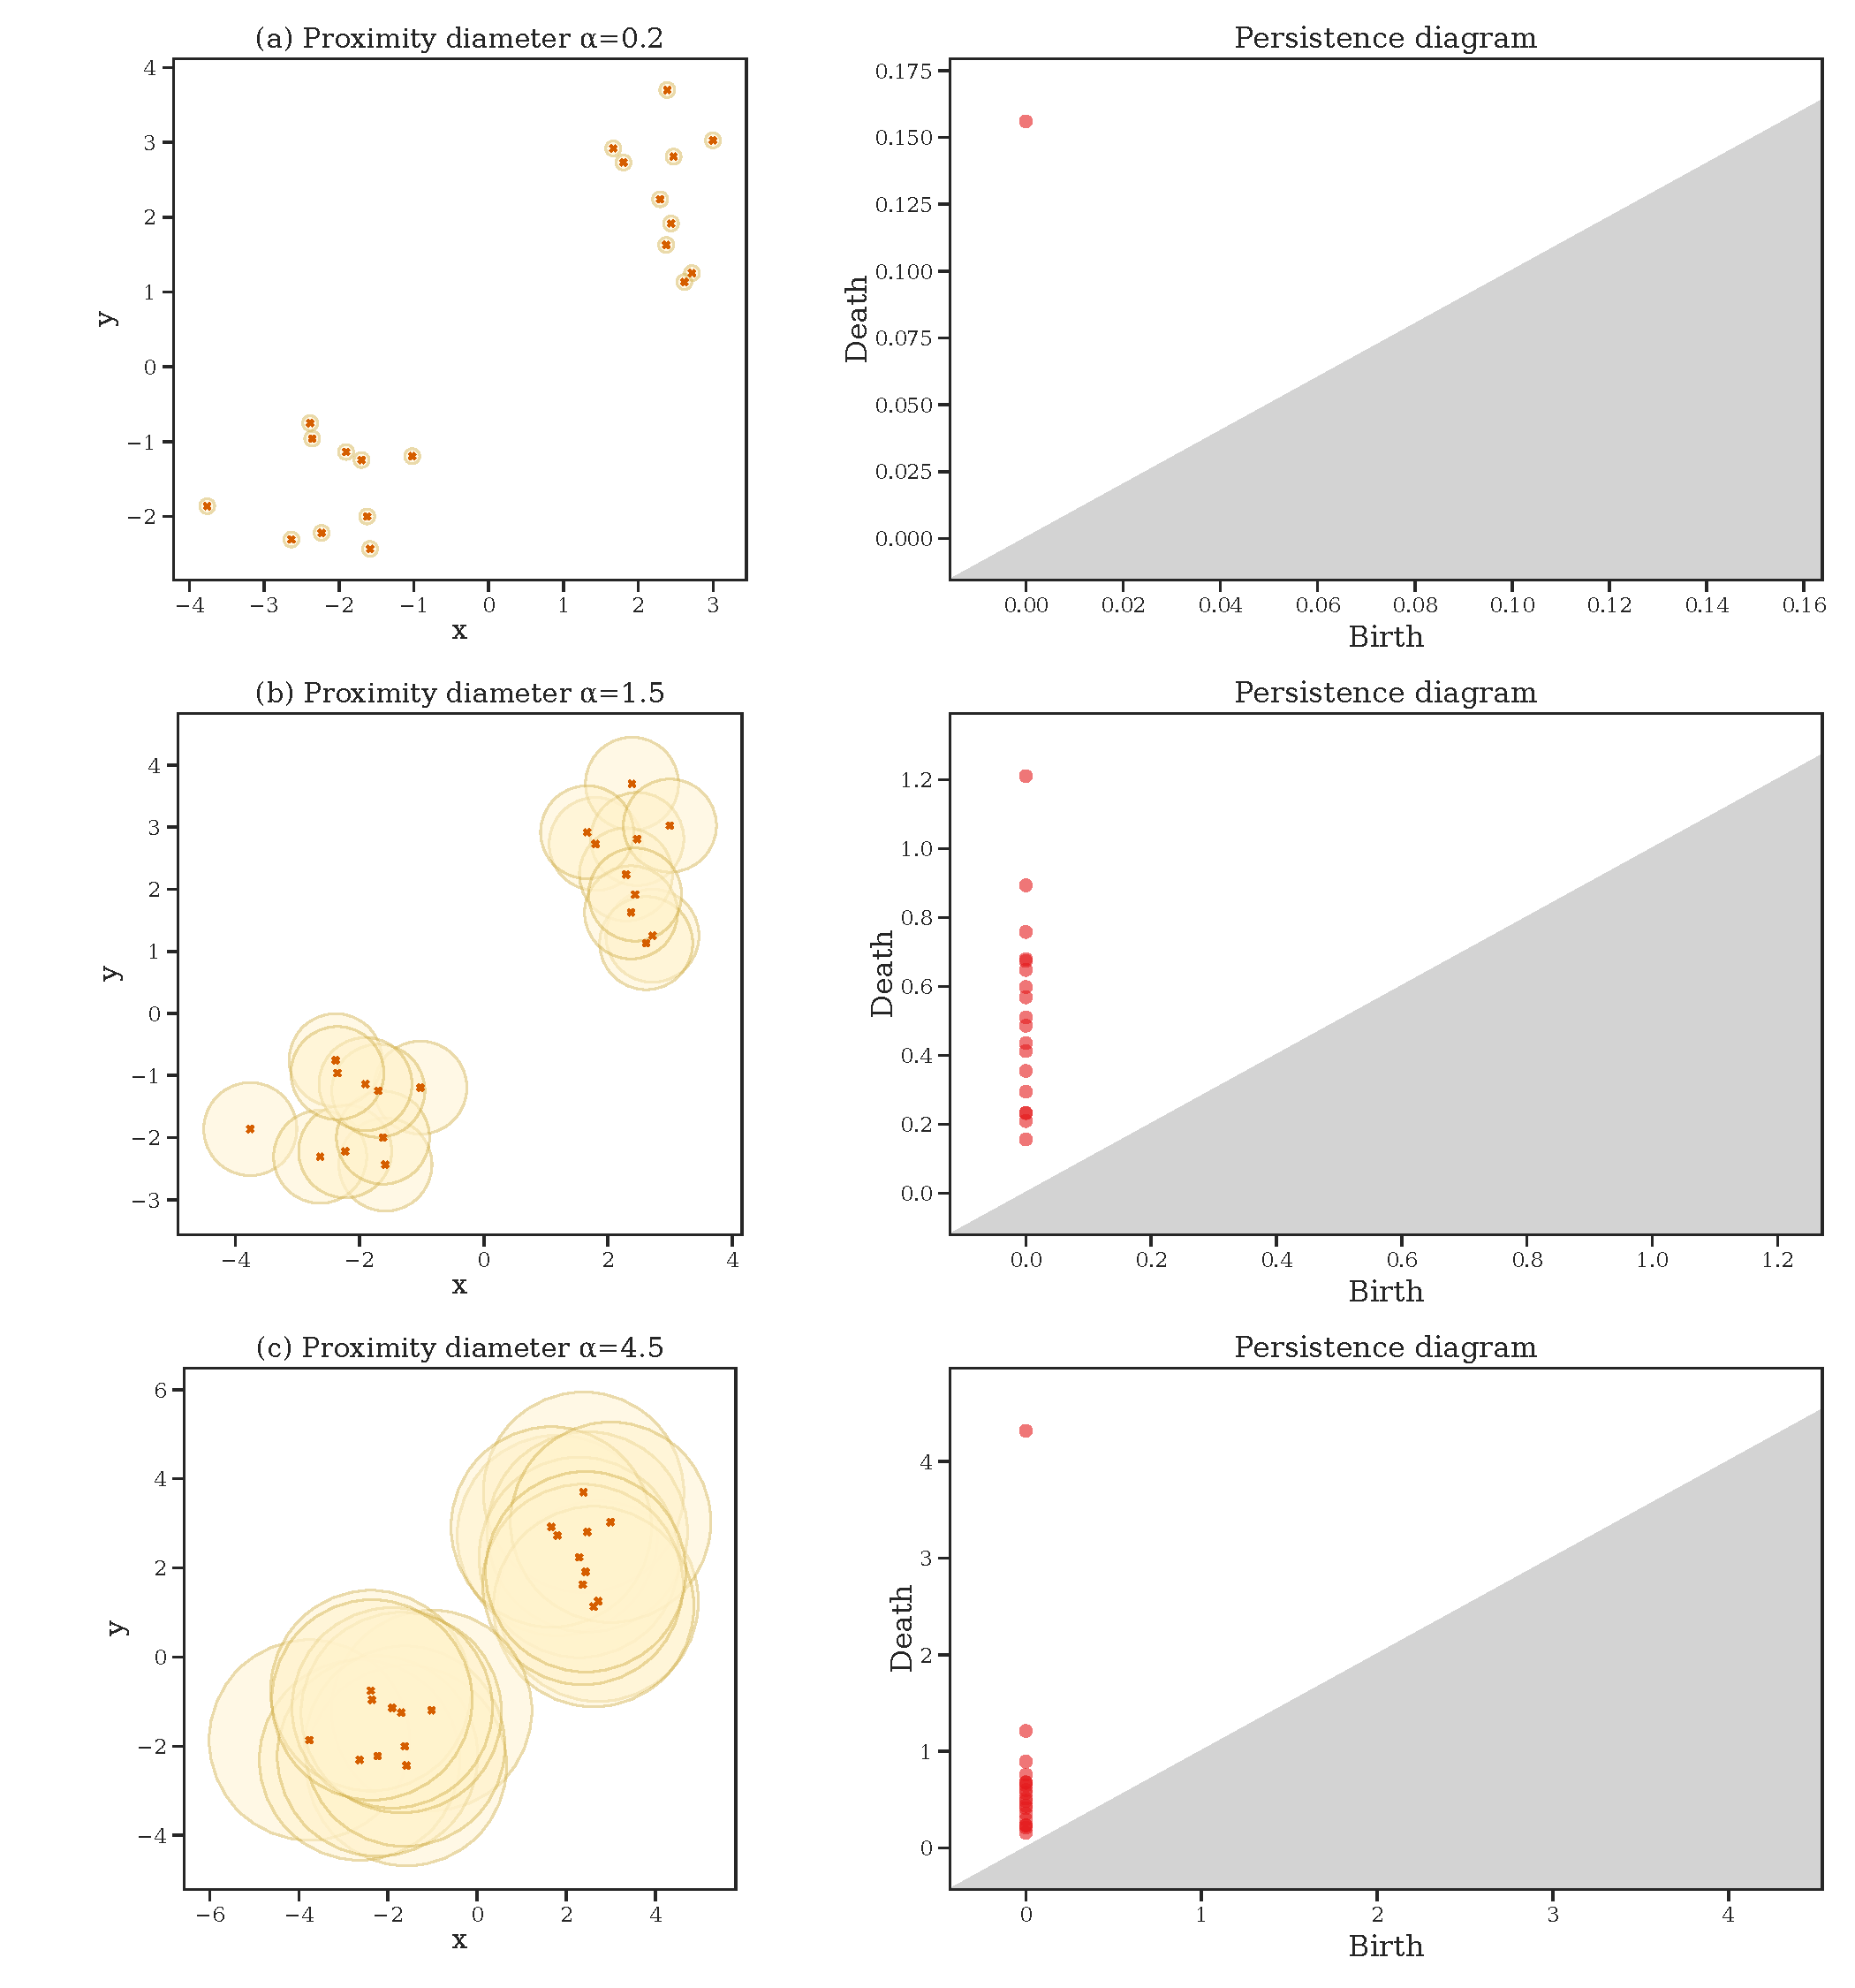
\includegraphics[width=1\textwidth]{thesis/figures/persistence-diagram-example.pdf}
    \caption{Persistence diagrams on different levels of $\alpha$ of a data set consisting of two blobs.}
    \label{fig:persistence-diagram-example}
\end{figure}
An important aspect of machine learning is to predict some quantity given some features. If we want to use the persistence diagrams as features in a model, for instance, a typical approach would be to perform some feature extraction or vectorization first. An example of vectorization of persistence diagrams is persistence images, which we introduce in the next subsection.

\subsection{Persistence image}
\label{sec:persistence-image}
Many machine learning tasks require valuable features to yield good results. \textit{Persistence images} \cite{adams2016persistence} are vector representations of persistence diagrams. When explaining persistence images, we refer to \cite{adams2016persistence}. Furthermore, we explain the use of persistence images for the analysis of word embeddings in \cref{sec:analysis-of-embeddings-geometric-anomaly-detection} and when discussing future work in \cref{chap:future-work}.

Let $B = \enclc{\enclp{b_1, d_1}, \enclp{b_2, d_2}, \ldots, \enclp{b_m, d_m}} \in \R^{m \times 2}$ be a persistence diagram in birth-death coordinates. First, we transform $B$ into birth-persistence coordinates, where \textit{persistence} is the difference between death and birth. That is, let $T(B) = \enclc{\enclp{b_1, p_1}, \enclp{b_2, p_2}, \ldots, \enclp{b_m, p_m}} \in \R^{m \times 2}$, where $p_i = b_i - d_i$ for $1 \leq i \leq m$. Following, for each of the point in the the $T(B)$ persistence diagram, we place a probability distribution. A common choice is to use the Gaussian distribution, which we center at each data point respectively. By placing probability distributions on each point, we are able to differentiate between dense and sparse areas. In addition to placing probability distributions on each point, we weight the distributions by the persistence of the point, making more persistent areas more prominent than others. Using the weighted probability distributions, for a particular persistence diagram $B$ we define the persistence surface of $\rho_B$ as
\begin{align}
    \rho_B(z) = \sumlim{u \in T(B)}{} f(u) \phi_u(z),
\end{align}
where $f(u)$ is the persistence weighing function and $\phi_u(z)$ is the probability distribution which we evaluate at point $z$ (e.g. if Gaussian, then we centre it at point $u$). Finally, we reduce the persistence surface $\rho_B(z)$ to a discretized representation. In particular, we form an $N \times M$ grid, and for each cell in the grid, we compute the integral of $\rho_B(z)$ over that region and use the result from the integral as value. In other words, this discretization allows us to summarize the persistence surface using less information and we are left with an $N \times M$ matrix which we can for machine learning tasks more easily. Finally, we illustrate the use of persistence images in \cref{fig:persistence-image-example}, where we apply it to a 2-dimensional data set consisting of two circles. In \cref{fig:persistence-image-example}, we see how the data is transformed into a persistence diagram $B$, following by the transformed persistence diagram $T(B)$ and finally the persistence image of $B$. In \cref{fig:persistence-image-example} (d), we see a 66 by 35 pixels image, representing the vectorization of persistence diagram $B$.
\begin{figure}[H]
    \centering
    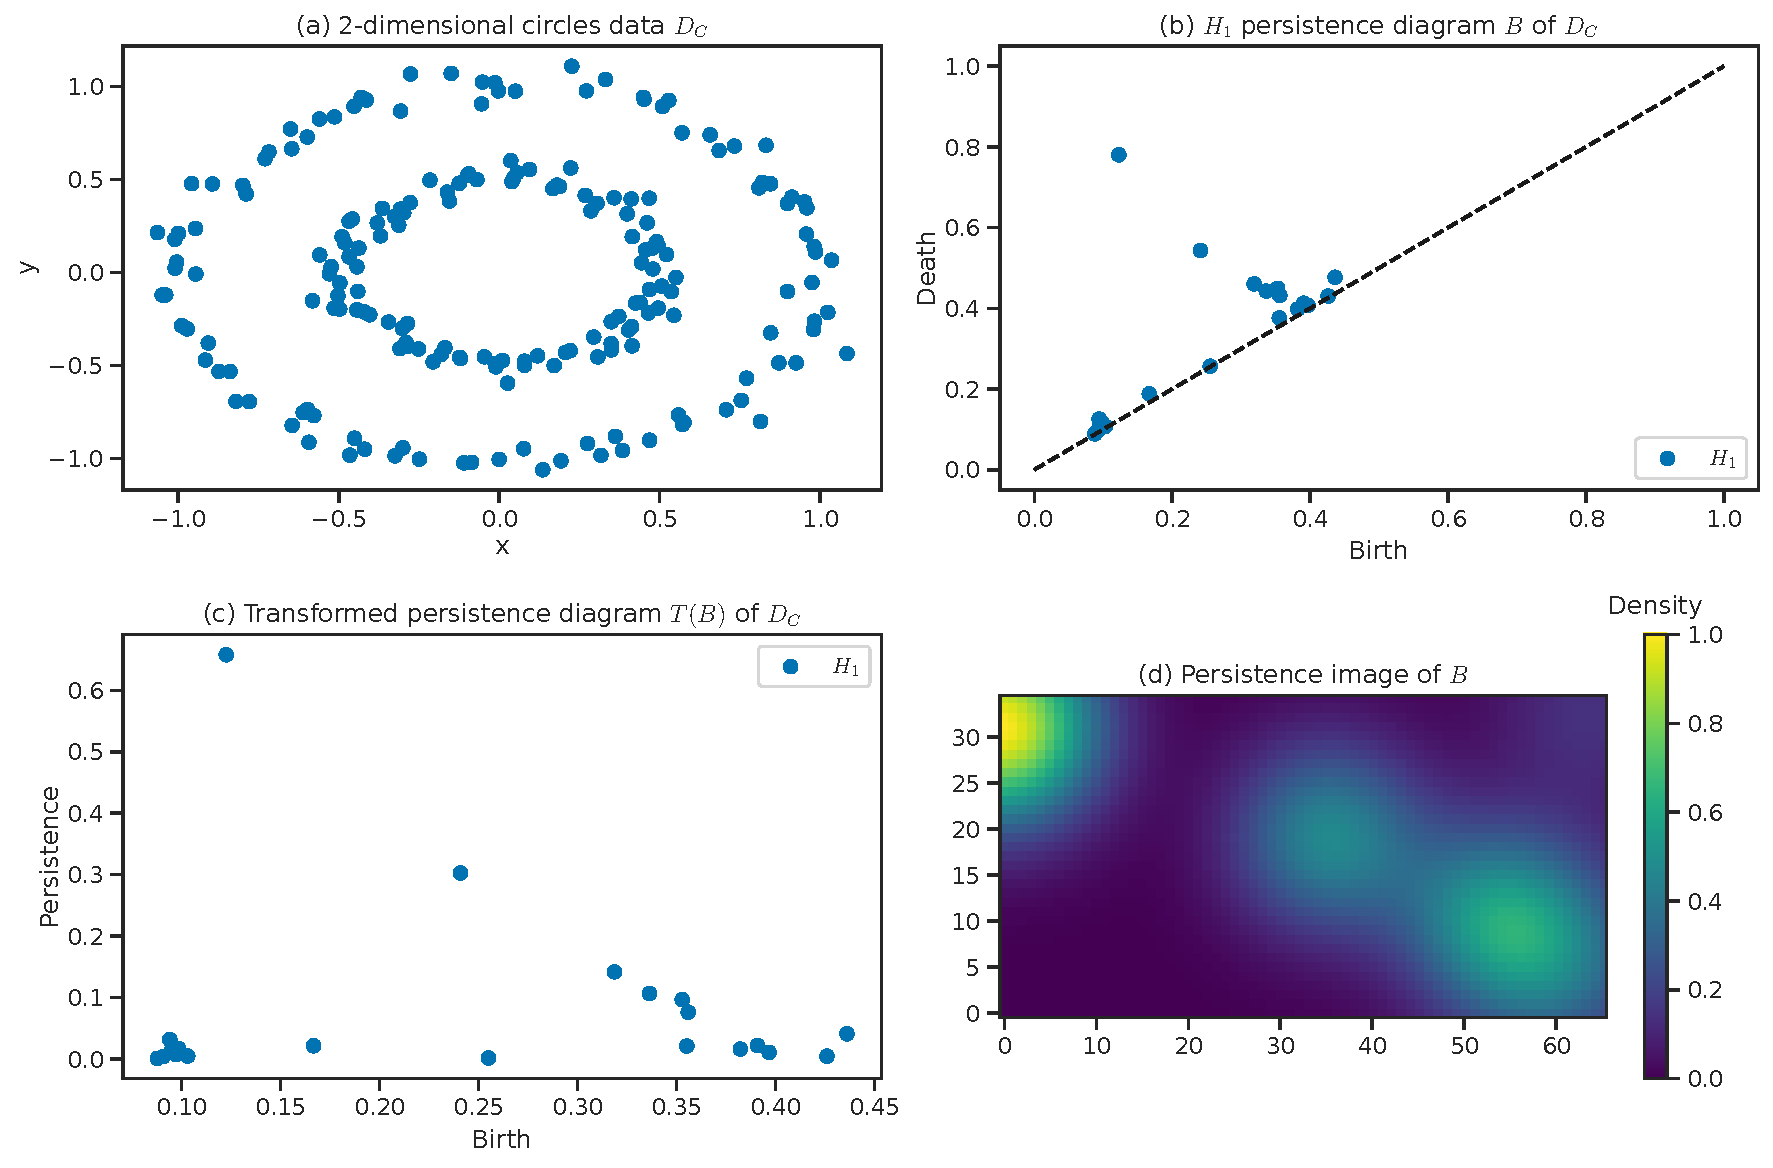
\includegraphics[width=\textwidth]{thesis/figures/persistence-image-example.pdf}
    \caption{Persistence image pipeline when applied to a 2-dimensional circles data set.}
    \label{fig:persistence-image-example}
\end{figure}

\subsection{Wasserstein distance}
\label{sec:wasserstein-distance}
When we compare distances between data points, we commonly use distance metrics (e.g. Euclidean distance). To compare differences between any two persistence diagrams $A$ and $B$, however, we use the $p$\textit{-Wasserstein distance}, which we define as
\begin{align}
    W_p(A, B) = \inf_{\gamma: A \rightarrow B} \enclp{\sumlim{u \in A}{} ||u - \gamma(u)||_{\infty}^{p}}^{1/p},
    \label{eqn:wasserstein-distance}
\end{align}
where $1 \leq p < \infty$ and $\gamma$ ranges over bijections between $A$ and $B$, and $\inf$ is the infimum (i.e. greatest lower bound; similar to "minimum"). We further visualize the idea behind the $p$-Wasserstein distance in \cref{fig:wasserstein-distance-example}, where we see how the points in each persistence diagram $A$ and $B$ get paired up. We match points to the diagonal if we find no matches for the particular point.
\begin{figure}[H]
    \centering
    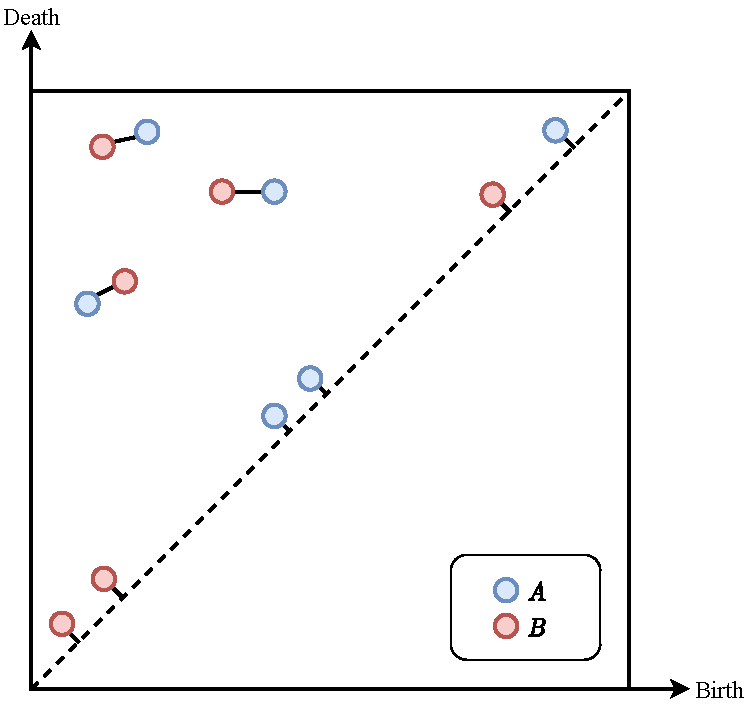
\includegraphics[width=0.7\textwidth]{thesis/figures/wasserstein-distance_cropped.pdf}
    \caption{$p$-Wasserstein distance between two persistence diagrams $A$ and $B$.}
    \label{fig:wasserstein-distance-example}
\end{figure}
Finally, if we let $p=\infty$, i.e $W_\infty(A, B)$, we get what we call the \textit{bottleneck distance}. We use the bottleneck distance to compare persistence diagrams as well. However, we note that the bottleneck distance has the disadvantage of only using the maximum distance between any two points over the bijections between $A$ and $B$.

\subsection{Topological polysemy}
\label{sec:topological-polysemy}
Recall the manifold hypothesis, which states that, in general, real-life high-dimensional data tends to live on a low-dimensional sub-manifold embedded within the high-dimensional space \cite[p. 16]{bengio2014representation}. To give an example, imagine that we some data about weight and height of humans. Naturally, we see that as the height increases, the weight increases as well. That is, we have a strong linear relationship (or correlation) between height and weight. We can therefore argue that the manifold dimension of the data is 1, even though the original data has dimension 2. The hypothesis should, in theory, also apply to word embeddings, but the authors of \cite{jakubowski2020topology} argue that word embeddings, should instead, live on a \textit{punched manifold}. By a pinched manifold, we mean a manifold where we "glue" together particular points that are equal in some sense, creating \textit{singular} areas in the manifold. We show an example of a pinched manifold in \cref{fig:pinched-manifold}, where we see an ideal pinched manifold for the word "solution" and four of its meanings as \textit{submanifolds}. For word embeddings, \cite{jakubowski2020topology} claim that these singular areas in the manifold represent polysemous words and that the neighbours of polysemous words share some relation to the polysemous word. To identify such polysemous words from word embeddings, \cite{jakubowski2020topology} introduce a topological measure of polysemy (using concepts from persistent homology) that correlates well with the true number of meanings of a word. To explain the topological measure of polysemy, we refer to \cite{jakubowski2020topology}.
\begin{figure}[H]
    \centering
    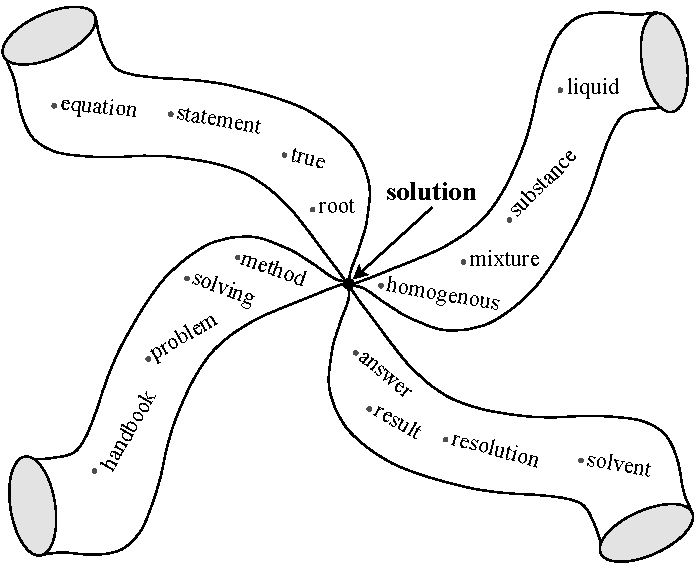
\includegraphics[width=0.7\textwidth]{thesis/figures/pinched-manifold_cropped.pdf}
    \caption{Pinched manifold of the word "solution", showing four of its meanings as submanifolds. This figure is inspired by \cite[Figure 5]{jakubowski2020topology}.}
    \label{fig:pinched-manifold}
\end{figure}

Determining the number of word meanings is a non-trivial task. Consider the word \textit{solution}, which has multiple meanings. In some contexts, the word \textit{solution} can relate to problem-solving (e.g. solving a problem in a handbook), while in other contexts, it can relate to chemistry (e.g. a mixture of two or more substances). We call such words \textit{polysemous}, meaning that the word has multiple meanings which can relate to one another. The opposite of a polysemous word is a \textit{monosemous} word, meaning that the word only has one meaning. The motivation behind the topological measure of polysemy, as introduced by \cite{jakubowski2020topology}, stamps from the fact that the number of components of a \textit{punctured neighbourhood} around a word $w$ should reflect the number of word meanings of the word $w$. A punctured neighbourhood of $w$ is the neighbouring words of $w$ excluding the word $w$ itself.

Let $W \in \R^{|V| \times d}$ be word embeddings, where $|V|$ is the number of words in the vocabulary and $d$ is the word embedding dimension. We compute the \textit{topological polysemy} $\text{TPS}_n(w)$ by fixing a target word $w$ and a neighbourhood size $n$. We denote the word vector of $w$ as $v_w \in \R^{d}$. To compute $\text{TPS}_n(w)$, we first normalize the word embeddings $W$ such that each vector are of unit length. We denote the normalized word embeddings as $W_\text{norm}$ and the normalized word vector of the target word $w$ as $v_{w_{\text{norm}}}$. Following, we compute the punctured neighbourhood $N_n(w)$, that is, the neighbouring $n$ normalized word vectors around $v_{w_{\text{norm}}}$, excluding $w$ itself. Furthermore, we project the word vectors of $N_n(w)$ to lie at the unit sphere, with $v_{w_{\text{norm}}}$ as the center. We denote this normalized punctured neighbourhood as $N'_n(w)$. In other words, we make the word vector of $w$ to be the origin of a $d$-dimensional sphere and project the neighbouring words of $w$ to lie around it. Lastly, we compute the 0-degree persistence diagram of $N'_n(w)$ and denote it as $PD_n(w)$. $\text{TPS}_n(w)$ is then the 1-Wasserstein distance (\cref{sec:wasserstein-distance}) between $PD_n(w)$ and the empty persistence diagram, also known as the Wasserstein norm. Furthermore, we will use topological polysemy later when analysing word embeddings in \cref{sec:analysis-of-embeddings-topological-polysemy} and for prediction of polysemous words in \cref{sec:analysis-of-embeddings-supervised-polysemy-prediction}.

\subsection{Geometric Anomaly Detection}
\label{sec:geometric-anomaly-detection}
The manifold hypothesis forms a foundation of modern data science. Many manifold learning and dimensionality reduction algorithms rely on this assumption to find meaningful low-dimensional representations of high-dimensional data. Examples of such algorithms include PCA (\cref{sec:pca}) and UMAP (\cref{sec:umap}). \textit{Geometric Anomaly Detection} (GAD) \cite{stolz2020geometric} is an algorithm for identifying possible points in data that fail to satisfy the manifold hypothesis. Following, we describe the GAD algorithm and give a couple of examples of how it works. We refer to \cite{stolz2020geometric} when explaining the GAD algorithm.

To understand how the GAD algorithm works, we first introduce the motivation behind it. Imagine that we have some data that lies on two submanifolds $P$ and $Q$. We illustrate such a situation in \cref{fig:gad-motivation}. Here we assume that the two submanifolds $P$ and $Q$ are planes that intersect at some point, which we mark by the dotted red line. We place an \textit{annulus} around each data point and infer its topological structure. An annulus is a region between two circles, where the first circle is contained in the other, and both circles share centre point. Annuli can also remind us of rings. Formally, each annulus around its respective data point has an inner radius $r$ and outer radius $s$. Depending on where a point is on either of the submanifolds, we observe that a point can have one of three states as seen in \cref{fig:gad-motivation} (a), (b) and (c). If a point is at the boundary of either submanifold, i.e. in \cref{fig:gad-motivation} (a), we observe that the points falling into the annulus around the data point forms a half-circle, as half of the circle does not have any data points in them. If we count the number of topological loops we get zero. If the data point falls nicely into either submanifold, i.e. in \cref{fig:gad-motivation} (b), we observe that we get a nice annulus where neighbouring points falling into the annulus around the data point forms a circle. In other words, if a point is on the submanifold, we expect to get exactly one topological loop. In the last situation, i.e. \cref{fig:gad-motivation} (c), we have a data point that falls between $P$ and $Q$, creating a singularity (or anomaly) in the data. This stamps from the fact that it is harder to distinguish which submanifold the particular data point should belong to. If we look at the data points in the annulus around the data point in \cref{fig:gad-motivation} (c), we observe that we get two or more topological loops.
\begin{figure}[H]
    \centering
    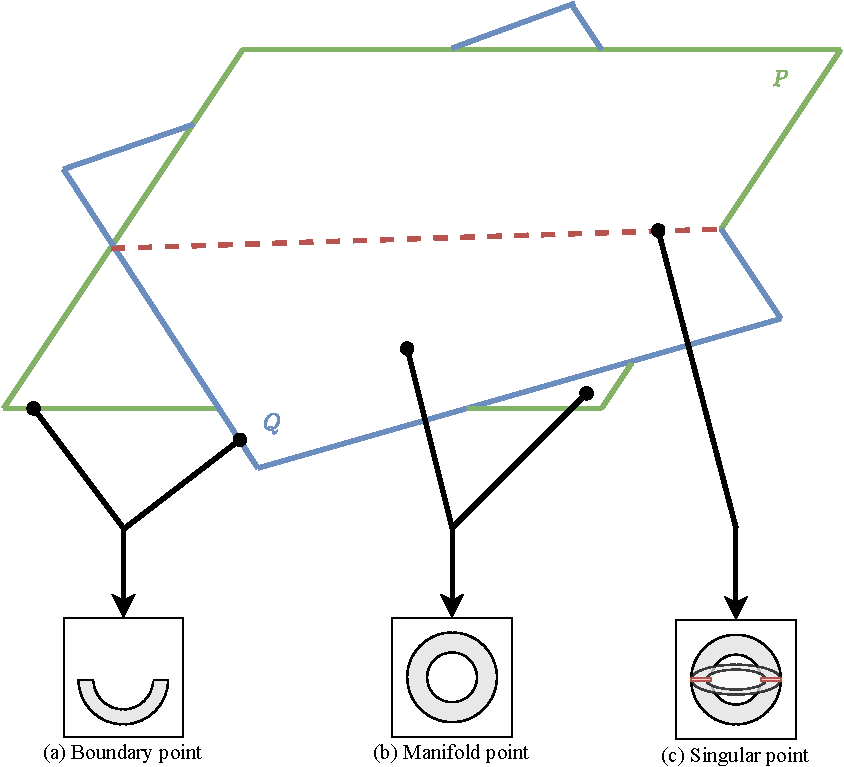
\includegraphics[width=0.8\textwidth]{thesis/figures/geometric-anomaly-detection-motivation_cropped.pdf}
    \caption{The motivation behind the GAD algorithm. Data points belonging to two submanifolds $P$ and $Q$, and depending on where the data points are on the submanifolds, it can have three different states: (a), (b) or (c). The GAD algorithm is particularly interested in finding singular (c) data points between $k$ submanifolds (here: $k=2$). This illustration is inspired by \cite[Figure 1]{stolz2020geometric}.}
    \label{fig:gad-motivation}
\end{figure}

Let $X \in R^{n \times d}$ be data points. The GAD algorithm works as follows: fix two parameters $0 < r < s$, and for each data point $x_i \in X$ place an annulus around it, with inner radius $r$ and outer radius $s$. Determine the data points that fall into the \textit{annular neighbourhood} of $x_i$ and denote this set as $A_y = \enclc{a_1, a_2, \ldots, a_m} \subset X$. That is, the set $A_y$ consists of those points $a_j$ that satisfies $r \leq d(x_i, g_j) \leq s$, where $d(\cdot, \cdot)$ measures the distance between two points (e.g. using Euclidean distance). Then, select a manifold dimension $k$ we would like to investigate, as the GAD algorithm discovers intersections of $(k-1)$ submanifolds. To find intersections of $(k-1)$ submanifolds of the annular neighbourhood $A_y$ of $x_i$, we compute the $(k-1)$-dimensional Vietoris–Rips complex of $A_y$, which we denote $VR_{k-1}(A_y)$. Then, for each birth-death coordinate $(b_{k-1}, d_{k-1}) \in VR_{k-1}(A_y)$, we count the number of points that persist longer as the annulus width. We denote this count as $N_y$. Recall that the persistence of points in persistence diagrams can be computed by transforming the persistence diagram into birth-persistence coordinates, where persistence $p_{k-1} = d_{k-1} - b_{k-1}$. We define the annulus width to be the difference between the outer and inner radius, i.e. $w_{A_y} = s - r$. To count $N_y$, we iterate over the points in the persistence diagram and count the number of points that satisfies
\begin{align}
    p_{k-1} > w_{A_y}.
    \label{eqn:gad-ny-condition}
\end{align}
The count $N_y$ is analogous to the number of topological loops that occur in $A_y$, for a particular homology dimension $(k-1)$. If no points satisfy \cref{eqn:gad-ny-condition}, i.e. $N_y=0$, then we classify $x_i$ as a boundary point, similar to the situation in \cref{fig:gad-motivation} (a). If we have exactly one point that satisfies \cref{eqn:gad-ny-condition}, i.e $N_y=1$, then we classify the point as a boundary point, similar to the situation in \cref{fig:gad-motivation} (b). If two or more points satisfy \cref{eqn:gad-ny-condition}, i.e. $N_y>1$, then we classify the point as a singular point, similar to the situation in \cref{fig:gad-motivation} (c). Furthermore, we will use GAD for later analysis of word embeddings in \cref{sec:analysis-of-embeddings-geometric-anomaly-detection} and for prediction of polysemous words in \cref{sec:analysis-of-embeddings-supervised-polysemy-prediction}. 